%%% Lecture 1 Slides %%%

\documentclass{beamer}

%\documentclass[handout]{beamer}
%\usepackage{pgfpages}
%\pgfpagesuselayout{2 on 1}[a4paper,border shrink=5mm]
%\pgfpagesuselayout{1 on 1}[a4paper,border shrink=5mm]



\usepackage{amssymb}
\usepackage{amsmath}


\newcommand{\bs}{\boldsymbol}
\newcommand{\mb}{\mathbf}
\newcommand{\indep}{{\bot\negthickspace\negthickspace\bot}}
\newcommand{\notindep}{{\bot\negthickspace\negthickspace\bot}{\negthinspace
  \negmedspace \negthickspace \negthickspace \diagup
  \;}}
\renewcommand{\S}{\mb{S}}

%\usepackage{pdfpages}
%\pdfpagelayout{2 on 1}

\mode<presentation>
{
  \usetheme{Singapore}    %Warsaw}
  % or ...

  \setbeamercovered{transparent}
  % or whatever (possibly just delete it)
}


\usepackage[english]{babel}
% or whatever

\usepackage[latin1]{inputenc}
% or whatever

\usepackage{times}
\usepackage[T1]{fontenc}
% Or whatever. Note that the encoding and the font should match. If T1
% does not look nice, try deleting the line with the fontenc.


\title[QTM 220] % (optional, use only with long paper titles)
{QTM 220}

\subtitle
{Regression with Randomized Experiments} 

\date{November 29, 2017}%[Short Occasion] % (optional)


\subject{Talks}

\AtBeginSection[]
{
  \begin{frame}<beamer>
    \frametitle{Outline}
    \tableofcontents[currentsection]
  \end{frame}
}


%\AtBeginSubsection[]
%{
%  \begin{frame}<beamer>
%    \frametitle{Outline}
%    \tableofcontents[currentsection,currentsubsection]
%  \end{frame}
%}


% If you wish to uncover everything in a step-wise fashion, uncomment
% the following command: 

%\beamerdefaultoverlayspecification{<+->}


\begin{document}

\begin{frame}
  \titlepage
\end{frame}

\begin{frame}
  \frametitle{Outline}
  \tableofcontents
  % You might wish to add the option [pausesections]
\end{frame}



\section{Simple Regression}

\frame{
\frametitle{Linear regression of $Y$ on $T$}

With binary $T$, the slope is a difference in means,

\begin{align*}
E[Y|T=t] &= \beta_0 + \beta_1 \cdot t \\
E[Y|T=0] &= \beta_0 \\
E[Y|T=1] &= \beta_0 + \beta_1 \\
\end{align*}\pause
and if the potential outcome are well defined such that $Y_i = T_i Y_i(1) + (1-T_i) Y_i(0)$ and $T$ has been randomized, 

\begin{align*}
\beta_1 &= E[Y_i|T_i=1] - E[Y_i|T_i=0] \\ 
&= E[Y_i(1)|T_i=1] - E[Y_i(0)|T_i=0] \\
&= E[Y_i(1)] - E[Y_i(0)] \\
&= E[Y_i(1) - Y_i(0)] 
\end{align*}

}

\frame{
\frametitle{What is the population?}

When the sample is a sample from a population
\begin{itemize}
\item the units of analysis are appoximately an i.i.d. sample from a population (e.g., some surveys)
\end{itemize} \pause

\vspace{.5cm}

When the sample is the population
\begin{itemize}
\item sample is all states in the country (e.g., effect of voter id laws on Trump vote share)
\item sample is all voters on the voters' register (e.g., effect of GOTV on turnout) 
\item sample is provisionally taken to be the population in order to focus first on internal validity (and postpone consideration of external validity)
\end{itemize}

}


\frame{
\frametitle{Point Estimation with Linear Regression}

If you have an i.i.d. sample, a binary treatment is randomized, and you run a linear regression of $Y$ on $T$, you get

\begin{itemize}
\item $\widehat{\beta}_1$ is an unbiased and consistent estimator of the ATE
\item because this is the ATE for the population (from which the i.i.d. sample comes), we sometime refer to it as the PATE (population average treatment effect)
\end{itemize} \pause

If instead the sample is the population, a binary treatment is randomized, and you run a linear regression of $Y$ on $T$, you get

\begin{itemize}
\item $\widehat{\beta}_1$ provides an unbiased estimator of the ATE
\item because the sample is the population, we sometime refer to as the ATE as the SATE (sample average treatment effect), and asymptotic concepts such as consistency are not applicable 
\end{itemize}

}



\frame{
\frametitle{Inference with an i.i.d. sample}

If you have an i.i.d. sample, a binary treatment is randomized, and you use robust standard errors or bootstrapping, then the CIs, tests, and $p$-values we developed for descriptive inference with a simple linear regression will be approximately correct. \\ \pause

\vspace{.8cm}

If homoskedasticity (constant conditional variance) also holds, then the CIs, tests, and $p$-values derived the $lm()$ function (or similar) will also will be approximately correct.

}


\frame{
\frametitle{Inference when sample is the population}

Because sample is the population, uncertainty due solely to random assignment of treatment. Fortunately, the CIs, tests, and $p$-values we developed for descriptive inference will be conservative in the sense that 

\vspace{.5cm}

\begin{itemize}
\item $(1-\alpha)\%$ CIs will have greater than $(1-\alpha)\%$ coverage.
\item $\alpha$ level tests will actually have probabilities of Type I error less than $\alpha$.
\item Reported $p$-values will be larger than the true $p$-values.
\item ... still need to worry about possible heteroskedasticity.
\end{itemize}


}



\begin{frame}[fragile]
\frametitle{Potential Outcomes and the Classical Econometric Linear Model}

\begin{align*}
Y_i &= T_i Y_i(1) + (1-T_i) Y_i(0)\\
&= Y_i(0) +  (Y_i(1)-Y_i(0)) T_i\\
&= \beta_{0i} + \beta_{1i} T_i \\
&= \beta_{0} + \beta_{1i} T_i + \epsilon_i
\end{align*}

If effects are constant across individuals (i.e., $\beta_{1i}=\beta_1$ for all $i$), then 
\begin{align*}
Y_i &= \beta_{0} + \beta_{1i} T_i + \epsilon_i\\
&= \beta_{0} + \beta_{1} T_i + \epsilon_i\\
\end{align*}
This is the linear model from ALZ page 125.

\end{frame}

\frame{
\frametitle{Unconfoundedness vs Errors Terms}

With the previous definitions and constant effects, we can re-write the potential outcomes as the following:
\begin{align*}
Y_i(1) &= \beta_{0} + \beta_{1} + \epsilon_i\\
Y_i(0) &= \beta_{0} + \epsilon_i\\
\end{align*}
This allows us to relate the unconfoundedness assumption to the classical error terms assumption.

\visible<1>{\begin{align*}
E[Y_i(1)] &= E[Y_i(1)|T=1] \\
 \beta_{0} + \beta_{1} + E[\epsilon_i] &= \beta_{0} + \beta_{1} + E[\epsilon_i|T=1] \\
\end{align*}}

\vspace{-2.9cm}

\visible<2>{\begin{align*}
E[Y_i(0)] &= E[Y_i(0)|T=1] \\
 \beta_{0} + E[\epsilon_i] &= \beta_{0} + E[\epsilon_i|T=1] \\
\end{align*}}


Therefore we have unconfoundedness when Assumption 5 from ALZ page 128 holds (i.e., $Cov(T_i, \epsilon_i)=0$ for all $i$)
}


\section{Multiple Regression}

\frame{
\frametitle{Recall: Randomization Implies Balance}

Suppose the subjects were randomly assigned to $T=0$ and $T=1$ (also imagine these six subjects actually represent 600 subjects), and we measure a ``pre-treatment'' covariate (i.e., not affected by $T$).  

\begin{center}
\begin{tabular}{cccc|ccc}
$i$ & $X_i$ &$T_i$ & $Y_i$ & $Y_i(1)$ & $Y_i(0)$ & $Y_i(1)-Y_i(0)$ \\
\hline
1 & 0  & 1 & 70 & 70 & ? & ? \\
2 & 1 & 1 & 80 & 80 & ? & ? \\
3 &  1& 0 & 60 & ? & 60 & ? \\
4 & 0  & 0 & 70 & ? & 70 & ? \\
5 &  0 & 0 & 70 & ? & 70 & ? \\
6 & 1 & 0 & 80 & ? & 80 & ? \\
\end{tabular}
\end{center}

Randomization implies that $X$ is independent of $T$, which implies that $E[X|T=1] = E[X|T=0]$.

}

\frame{
\frametitle{Balance on Pre-treatment Variables in the Gerber, Green, and Larimer Experiment}

\begin{center}
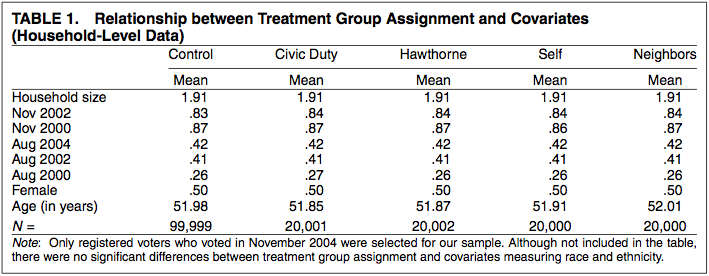
\includegraphics[width=4in]{GGL}
\end{center}

}

\frame{
\frametitle{Why balance in large samples?}


\begin{center}
\begin{tabular}{cccc|ccc}
$i$ & $X_i$ &$T_i$ & $Y_i$ & $Y_i(1)$ & $Y_i(0)$ & $Y_i(1)-Y_i(0)$ \\
\hline
1 & 0  & 1 & 70 & 70 & ? & ? \\
2 & 1 & 1 & 80 & 80 & ? & ? \\
3 &  1& 0 & 60 & ? & 60 & ? \\
4 & 0  & 0 & 70 & ? & 70 & ? \\
5 &  0 & 0 & 70 & ? & 70 & ? \\
6 & 1 & 0 & 80 & ? & 80 & ? \\
\end{tabular}
\end{center}

\begin{itemize}
\item The $T=1$ rows are a random sample of the rows, therefore $E[X|T=1] = E[X]$. 
\item The $T=0$ rows are a random sample of the rows, therefore $E[X|T=0] = E[X]$.
\item Therefore $E[X|T=1] = E[X|T=0]$.
\end{itemize}

}

\frame{
\frametitle{Warning: Balance only for pre-treatment X}

\begin{itemize}
\item If $X$ is affected by $T$, then the previous results will not hold
\item Even though the $T=1$ rows are a random sample of the rows, $E[X|T=1] \ne E[X]$. 
\item Even though the $T=0$ rows are a random sample of the rows, $E[X|T=0] \ne E[X]$.
\item Therefore $E[X|T=1] \ne E[X|T=0]$.
\item Suppose $Y$ indicates a heart attack, $T$ is a blood pressure medicine, and $X$ is blood pressure.
\end{itemize}

}

\begin{frame}[fragile]
\frametitle{Recall: What if $x$ and $z$ are uncorrelated?}

\begin{verbatim}
> z <- rnorm(n)
> x <- rnorm(n) # no z
> cor(x,z)
[1] 0.01075281
> y <- x + z + rnorm(n)
> lm(y ~ x)
Coefficients:
(Intercept)            x  
    0.01027      1.00940  

> lm(y ~ x + z)

Coefficients:
(Intercept)            x            z  
    0.00417      0.99901      0.98509  
    \end{verbatim}

\end{frame}


\frame{
\frametitle{Including Covariates in the Gerber, Green, and Larimer Experiment}

\begin{center}
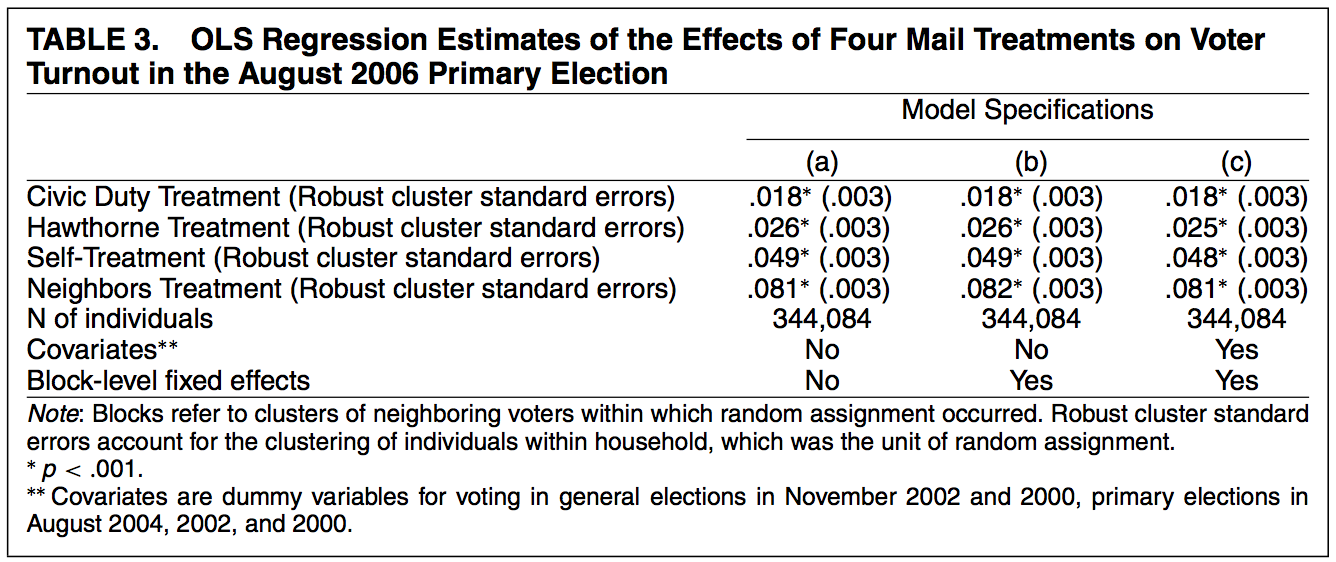
\includegraphics[width=4in]{GGL2}
\end{center}

}

\frame{
\frametitle{Simple vs Additive Multiple Linear Regression Analysis of Randomized Experiments}

\begin{itemize}
\item In very large samples, additive multiple linear regression will produce approximately the same answer as simple linear regression for the ATE (e.g., social pressure). \pause
\item In medium/large samples, ($> 30$ d.f.), multiple linear regression will have small bias but will generally more efficient than simple linear regression. %Sufficient condition:
%$$
%\frac{Cov(Y_i(0),X_i)}{V(X_i)} + \frac{Cov(Y_i(1),X_i)}{V(X_i)} > 1
%$$
\pause
\item In small samples, the bias in multiple linear regression will be too much.  
\end{itemize}


}

\frame{
\frametitle{Interpreting the Multiple Regression Model}

Consider the multiple regression model from ALZ page 158.
\visible<1>{\begin{align*}
Y_i &= \beta_{0} + \beta_{1} X_{1i} + \beta_{2} X_{2i} + \dots +  \beta_{k} X_{ki}  + \epsilon_i
\end{align*}}

\vspace{-2cm}

\visible<2->{\begin{align*}
Y_i &= \beta_{0} + \beta_{1} X_{1i} + \beta_{2} X_{2i} + \epsilon_i
\end{align*}}

\begin{itemize}
\item<3->  Should we interpret both $\beta_{1}$ and $\beta_{2}$ as causal effects?
%\item<4->  If so, would this interpretation be justified if $X_{1}$ were randomized conditionally on $X_{2}$?
\item<4->  What randomized experiment would justify this interpretation?
\end{itemize}


}

%\begin{frame}[fragile]
%\frametitle{Recall Potential Outcomes and the Classical Model}
%
%\begin{align*}
%Y_i &= T_i Y_i(1) + (1-T_i) Y_i(0)\\
%&= Y_i(0) +  (Y_i(1)-Y_i(0)) T_i\\
%&= \beta_{0i} + \beta_{1i} T_i \\
%&= \beta_{0} + \beta_{1i} T_i + \epsilon_i
%\end{align*}
%
%If effects are constant across individuals (i.e., $\beta_{1i}=\beta_1$ for all $i$), then 
%\begin{align*}
%Y_i &= \beta_{0} + \beta_{1i} T_i + \epsilon_i\\
%&= \beta_{0} + \beta_{1} T_i + \epsilon_i\\
%\end{align*}
%This is the linear model from ALZ page 125.
%
%\end{frame}
%
%\frame{
%\frametitle{Unconfoundedness vs Errors Terms}
%
%With the previous definitions and constant effects, we can re-write the potential outcomes as the following:
%\begin{align*}
%Y_i(1) &= \beta_{0} + \beta_{1} + \epsilon_i\\
%Y_i(0) &= \beta_{0} + \epsilon_i\\
%\end{align*}
%This allows us to relate the conditional exchangeability/unconfoundedness assumption to the classical error terms assumption.
%
%\visible<1>{\begin{align*}
%E[Y_i(1)|X=x] &= E[Y_i(1)|T=1,X=x] \\
% \beta_{0} + \beta_{1} + E[\epsilon_i|X=x] &= \beta_{0} + \beta_{1} + E[\epsilon_i|T=1,X=x] \\
%\end{align*}}
%
%\vspace{-2.9cm}
%
%\visible<2>{\begin{align*}
%E[Y_i(0)|X=x] &= E[Y_i(0)|T=1,X=x] \\
% \beta_{0} + E[\epsilon_i|X=x] &= \beta_{0} + E[\epsilon_i|T=1,X=x] \\
%\end{align*}}
%
%
%%Therefore we have unconfoundedness when Assumption 5 from ALZ page 128 holds (i.e., $Cov(T_i, \epsilon_i)=0$ for all $i$)
%}


\section{Interactive Regression}

\frame{
\frametitle{CATEs}


With a randomized experiment, the unconfoundedness assumption will hold conditional on any set of pre-treatment covariates ($X$).


\visible<1->{\begin{align*}
E[Y_i(1)|X=x] &= E[Y_i(1)|T_i=1,X_i=x] \\
&= E[Y_i|T_i=1,X_i=x]
\end{align*}}

%\vspace{-2.9cm}

\visible<2->{\begin{align*}
E[Y_i(0)|X_i=x] &= E[Y_i(0)|T_i=0,X_i=x] \\
&= E[Y_i(0)|T_i=0,X_i=x]
\end{align*}}

\visible<3>{
Conditional Average Treatment Effect (CATE)
\begin{align*}
E[Y_i(1) - &Y_i(0)|X_i=x]
%&E_X\{ E[Y_i|T_i=1,X_i=x] - E[Y_i|T_i=0,X_i=x]\} 
\end{align*}}

}

\frame{
\frametitle{CATE examples}

\begin{itemize}
\item average effect among men/average effect among women
\item average effect among those with annual income of 15k,16k,17k,18k,....
\item average effect among low/high propensity voters
\end{itemize}


}

\frame{
\frametitle{Estimating CATEs with Interactions}

With a binary $T$ and a binary $X$, we can always write the conditional expectation as a linear interactive function,

\begin{align*}
E[Y|T=t,X=x] &= \beta_0 + \beta_1 \cdot t + \beta_2 \cdot x + \beta_3 \cdot t \cdot x \\
\visible<2->{E[Y|T=0,X=0] &= \beta_0} \\
\visible<3->{E[Y|T=1,X=0] &= \beta_0 + \beta_1} \\
\visible<4->{E[Y|T=0,X=1] &= \beta_0 + \beta_2} \\
\visible<5->{E[Y|T=1,X=1] &= \beta_0 + \beta_1 + \beta_2 + \beta_3}
\end{align*}


}

\frame{
\frametitle{Interpretation with Interactive Model}

Therefore, with an interactive model,
\begin{align*}
E[Y|T=1,X=0]-E[Y|T=0,X=0] &= (\beta_0 + \beta_1) - \beta_0 \\
&= \beta_1
\end{align*}
can be interpreted as the CATE among the $X=0$ subjects. \pause
\begin{align*}
E[Y|T=1,X=1]&-E[Y|T=0,X=1] = \\
&(\beta_0 + \beta_1 + \beta_2 + \beta_3) - (\beta_0 + \beta_2) \\
&= \beta_1+\beta_3
\end{align*}
can be interpreted as the CATE among the $X=1$ subjects. \pause
\begin{align*}
E[ \beta_1+\beta_3 \cdot X] &= \beta_1+\beta_3 \cdot E[X]\\
&= (1-E[X]) \beta_1 +  E[X] (\beta_1+\beta_3)
\end{align*}
can be interpreted as the ATE 


}

\frame{
\frametitle{Interpretation with Interactive Model (non-binary $X$)}

With non-binary $X$, a linear interactive model requires a linearity assumption
\begin{align*}
E[Y|T=t,X=x] &= \beta_0 + \beta_1 \cdot t + \beta_2 \cdot x + \beta_3 \cdot t \cdot x  \\
&= \beta_0 + \beta_2 \cdot x + (\beta_1 + \beta_3 \cdot x) \cdot t \\
\end{align*}
where $(\beta_1 + \beta_3 \cdot x)$ can be interpreted as the CATE among the $X=x$ subjects.  \pause

And the ATE can still be recovered in the following way
\begin{align*}
E[ \beta_1+\beta_3 \cdot X] &= \beta_1+\beta_3 \cdot E[X]
\end{align*}
... more complicated for non-linear models.


}



\section{Logistic Regression}

\frame{
\frametitle{Recall: CATEs}


With a randomized experiment, the unconfoundedness assumption will hold conditional on any set of pre-treatment covariates ($X$).


\visible<1->{\begin{align*}
E[Y_i(1)|X=x] &= E[Y_i(1)|T_i=1,X_i=x] \\
&= E[Y_i|T_i=1,X_i=x]
\end{align*}}

%\vspace{-2.9cm}

\visible<2->{\begin{align*}
E[Y_i(0)|X_i=x] &= E[Y_i(0)|T_i=0,X_i=x] \\
&= E[Y_i|T_i=0,X_i=x]
\end{align*}}

\visible<3>{
Conditional Average Treatment Effect (CATE)
\begin{align*}
E[Y_i(1) - &Y_i(0)|X_i=x]
%&E_X\{ E[Y_i|T_i=1,X_i=x] - E[Y_i|T_i=0,X_i=x]\} 
\end{align*}}

}

\frame{
\frametitle{CATEs with Additive Linear Regression}


\visible<1->{\begin{align*}
E[Y_i(1)|X=x] &= E[Y_i(1)|T_i=1,X_i=x] \\
&= E[Y_i|T_i=1,X_i=x] \\
&=  \beta_0 + \beta_1 \cdot 1 + \beta_2 \cdot x 
\end{align*}}

\vspace{-.5cm}

\visible<2->{\begin{align*}
E[Y_i(0)|X_i=x] &= E[Y_i(0)|T_i=0,X_i=x] \\
&= E[Y_i|T_i=0,X_i=x]\\
&=  \beta_0 + \beta_1 \cdot 0 + \beta_2 \cdot x 
\end{align*}}

\visible<3>{
Conditional Average Treatment Effect (CATE)
\begin{align*}
E[Y_i|T_i=1,X_i=x] -E[Y_i|T_i=0,X_i=x] =  \beta_1
%&E_X\{ E[Y_i|T_i=1,X_i=x] - E[Y_i|T_i=0,X_i=x]\} 
\end{align*}}

}

\frame{
\frametitle{CATEs with Interactive Linear Regression}


\visible<1->{\begin{align*}
E[Y_i(1)|X=x] &= E[Y_i(1)|T_i=1,X_i=x] \\
&= E[Y_i|T_i=1,X_i=x] \\
&=  \beta_0 + \beta_1 \cdot 1 + \beta_2 \cdot x + \beta_3 \cdot 1 \cdot x
\end{align*}}

\vspace{-.5cm}

\visible<2->{\begin{align*}
E[Y_i(0)|X_i=x] &= E[Y_i(0)|T_i=0,X_i=x] \\
&= E[Y_i|T_i=0,X_i=x]\\
&=  \beta_0 + \beta_1 \cdot 0 + \beta_2 \cdot x + \beta_3 \cdot 0 \cdot x
\end{align*}}

\visible<3>{
Conditional Average Treatment Effect (CATE)
\begin{align*}
E[Y_i|T_i=1,X_i=x] -E[Y_i|T_i=0,X_i=x] =  \beta_1 + \beta_3 x
%&E_X\{ E[Y_i|T_i=1,X_i=x] - E[Y_i|T_i=0,X_i=x]\} 
\end{align*}}

}

\frame{
\frametitle{CATEs with Logistic Regression}


\visible<1->{\begin{align*}
E[Y_i(1)|X=x] &= E[Y_i(1)|T_i=1,X_i=x] \\
&= E[Y_i|T_i=1,X_i=x] \\
&=  \frac{\exp(\beta_0 + \beta_1 \cdot 1 + \beta_2 \cdot x)}{1+\exp(\beta_0 + \beta_1 \cdot 1 + \beta_2 \cdot x)}
\end{align*}}

\vspace{-.5cm}

\visible<2->{\begin{align*}
E[Y_i(0)|X_i=x] &= E[Y_i(0)|T_i=0,X_i=x] \\
&= E[Y_i|T_i=0,X_i=x]\\
&=   \frac{\exp(\beta_0 + \beta_1 \cdot 0 + \beta_2 \cdot x)}{1+\exp(\beta_0 + \beta_1 \cdot 0 + \beta_2 \cdot x)}
\end{align*}}

\visible<3>{
Conditional Average Treatment Effect (CATE)
\begin{align*}
E[Y_i|T_i=1,X_i=x] -E[Y_i|T_i=0,X_i=x] =  \\
 \frac{\exp(\beta_0 + \beta_1 \cdot 1 + \beta_2 \cdot x)}{1+\exp(\beta_0 + \beta_1 \cdot 1 + \beta_2 \cdot x)}
- \frac{\exp(\beta_0 + \beta_1 \cdot 0 + \beta_2 \cdot x)}{1+\exp(\beta_0 + \beta_1 \cdot 0 + \beta_2 \cdot x)}
%&E_X\{ E[Y_i|T_i=1,X_i=x] - E[Y_i|T_i=0,X_i=x]\} 
\end{align*}}

}

\frame{
\frametitle{ATEs with Logistic Regression}
An ATE can be recovered in the following way
\begin{align*}
E_X[ \frac{\exp(\beta_0 + \beta_1 \cdot 1 + \beta_2 \cdot x)}{1+\exp(\beta_0 + \beta_1 \cdot 1 + \beta_2 \cdot x)} - \frac{\exp(\beta_0 + \beta_1 \cdot 0 + \beta_2 \cdot x)}{1+\exp(\beta_0 + \beta_1 \cdot 0 + \beta_2 \cdot x)}]
\end{align*}

}

\frame{
\frametitle{Estimating ATEs with Logistic Regression}


\begin{align*}
\widehat{ATE} &= \frac{1}{n} \sum_i^n \frac{\exp(\hat \beta_0 + \hat \beta_1 \cdot 1+ \hat \beta_2  \cdot  x_i )}{1+\exp(\hat \beta_0 + \hat \beta_1 \cdot 1+ \hat \beta_2  \cdot  x_i )}  \\
&- \frac{1}{n} \sum_i^n \frac{\exp(\hat \beta_0 + \hat \beta_1 \cdot 0+ \hat \beta_2  \cdot  x_i )}{1+\exp(\hat \beta_0 + \hat \beta_1 \cdot 0+ \hat \beta_2  \cdot  x_i )}
\end{align*}

How would you do this in $R$? Standard errors?

}


\frame{
\frametitle{CATEs and ATEs with other}


\visible<1->{\begin{align*}
E[Y_i(1)|X=x] &= E[Y_i(1)|T_i=1,X_i=x] \\
&= E[Y_i|T_i=1,X_i=x] \\
&=  ?
\end{align*}}

\vspace{-.5cm}

\visible<2->{\begin{align*}
E[Y_i(0)|X_i=x] &= E[Y_i(0)|T_i=0,X_i=x] \\
&= E[Y_i|T_i=0,X_i=x]\\
&=   ?
\end{align*}}

\visible<3>{
\begin{align*}
E_X[ ?]
\end{align*}
}

}





\end{document}




%%%%%%%%%%%%%%%%%%%%%%%%%%%%%%

